\documentclass[11pt,letterpaper]{article}
\usepackage[lmargin=1in,rmargin=1in,tmargin=1in,bmargin=1in]{geometry}
\usepackage{../style/homework}
\usepackage{../style/commands}
\setbool{quotetype}{true} % True: Side; False: Under
\setbool{hideans}{false} % Student: True; Instructor: False

% -------------------
% Content
% -------------------
\begin{document}

\homework{3: Due 09/18}{Fire can't go through doors, stupid. It's not a ghost.}{Ben Chang, Community}

% Problem 1
\problem{10} Consider the triangle given below:
	\[
	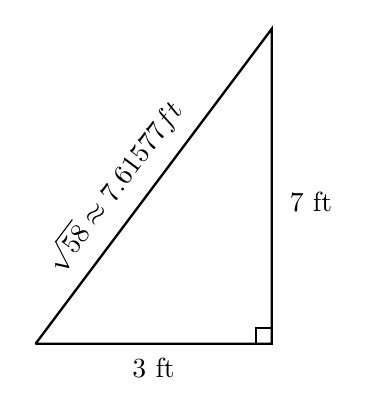
\begin{tikzpicture}
	\draw[line width=0.03cm] (0,0) -- (3,0) -- (3,4) -- (0,0);
	\draw[line width=0.03cm] (2.8,0) -- (2.8,0.2) -- (3,0.2);
	\node at (1.5,-0.3) {$3$~ft};
	\node at (3.5,1.8) {$7$~ft};
	
	\node[rotate=53.1301] at (1,2) {$\sqrt{58} \approx 7.61577 \text{ ft}$};
	\end{tikzpicture}
	\]

\begin{enumerate}[(a)]
\item Find the perimeter of the triangle.
\item Find the area of the triangle. 
\item If the lengths of the legs in the triangle were mislabeled as being in feet when they should have been in meters, convert your answer in (b) to square meters. 
\end{enumerate} 

\sol 
\begin{enumerate}[(a)]
\item To find the perimeter of the triangle, we first need to find the length of the hypotenuse. Using the Pythagorean Theorem, $a^2 + b^2= c^2$, we have\dots
	\[
	\begin{gathered}
	c^2= a^2 + b^2 \\
	c^2= (3 \text{ ft})^2 + (7 \text{ ft})^2 \\
	c^2= 9 \text{ ft}^2 + 49 \text{ ft}^2 \\
	c^2= 58 \text{ ft}^2 \\
	c= \sqrt{58} \text{ ft} \approx 7.61577 \text{ ft}
	\end{gathered}
	\]
We know that the perimeter of the triangle is the sum of the lengths of its sides, i.e. $P= a + b + c$. But then\dots
	\[
	P= a + b + c= 3 \text{ ft} + 7 \text{ ft} + 7.61577 \text{ ft}= 17.61577 \text{ ft}
	\]

\item We know that the area of a triangle is $A= \frac{1}{2} \cdot \text{base} \cdot \text{height}$. But then we have $A= \frac{1}{2} \cdot 3 \text{ ft} \cdot 7 \text{ ft}= \frac{21}{2} \text{ ft}^2 = 10.5 \text{ ft}^2$. 

\item We have\dots \par
	\begin{table}[H]
	\centering
	\begin{tabular}{c||c|c}
	10.5~ft$^2$ & 1~m & 1~m \\ \hline
			   & 3.28084~ft & 3.28084~ft
	\end{tabular} = 0.975482~m$^2$
	\end{table} \par
Alternatively, we can convert each of the lengths of legs of the triangle to meters. The legs with length 3~ft and 7~ft in meters are 0.9143~m and 2.1336~m, respectively. But then the area of the triangle is $A= \frac{1}{2} \cdot 0.9143 \text{ m} \cdot 2.1336 \text{ m}=  0.975375 \text{ m}^2$, as obtained above. 
\end{enumerate}



\newpage



% Problem 2
\problem{10} Consider the `track' shown below:
	\[
	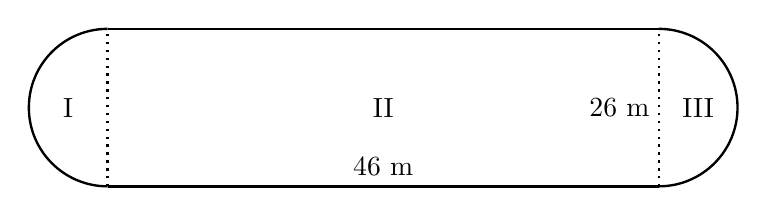
\begin{tikzpicture}
	\draw[line width=0.03cm] (0,0) -- (7,0);
	\draw[line width=0.03cm] (0,2) -- (7,2);
	
	\draw[line width=0.03cm,dotted] (0,0) -- (0,2);
	\draw[line width=0.03cm,dotted] (7,0) -- (7,2);
	 
	\draw[line width=0.03cm] (0,2) arc(90:270:1);
	\draw[line width=0.03cm] (7,0) arc(270:450:1);
	
	\node at (3.5,0.25) {$46$~m};
	\node at (6.5,1) {$26$~m};
	
	\node at (-0.5,1) {I};
	\node at (3.5,1) {II};
	\node at (7.5,1) {III};
	\end{tikzpicture}
	\]

\begin{enumerate}[(a)]
\item Find the perimeter of the track.
\item Find the area of the track.
\item If you scale the track's size by a factor of two, what is the new perimeter and area?
\item Suppose you were going to tile the interior rectangular portion of the track with special 2~m $\times$ 2~m tiles. How many tiles would you need?
\end{enumerate} \pspace

\sol 
\begin{enumerate}[(a)]
\item The perimeter of the track is the distance around the track. This will be the distance along the upper and lower `straightaways' along with the two half circles. The distance around a circle is its circumference. The circumference of a circle is $C= \pi d$, where $d$ is the diameter of the circle. The diameter of the circles above is 26~m. However, each is only a half circle, i.e. $\frac{1}{2}C= \frac{\pi d}{2}$. Therefore, we have\dots\footnote{Observe that we can `combine' the half-circles into one full-circle and the two `straightaways' into one that is twice as long. But then the perimeter is $P= 2 \cdot 46 \text{ m} + \pi \cdot 26 \text{ m}= 92 \text{ m} + 26 \pi \text{ m}$.}
	\[
	P= 46 \text{ m} + \dfrac{\pi \cdot 26 \text{ m}}{2} + 46 \text{ m} + \dfrac{\pi \cdot 26 \text{ m}}{2}= 46 \text{ m} + 46 \text{ m} + 13\pi \text{ m} + 13 \pi \text{ m}= 92 \text{ m} + 26 \pi \text{ m} \approx 173.7 \text{ m}
	\] \pspace

\item Break the track into regions I, II, and III, as labeled in the diagram above. Region~II is a rectangle and regions~I and III are half-circles. The area of a rectangle is $A= \ell w$, where $\ell$ is the length and $w$ is the width. The area of a circle is $A= \pi r^2$, where $r$ is the radius of the circle. Then the area of a half-circle is $\frac{1}{2}A= \frac{\pi r^2}{2}$. The radii of half-circles I and II are clearly $r= \frac{d}{2}= \frac{26 \text{ m}}{2}= 13 \text{ m}$. Therefore, we have\dots\footnote{Just as with (a), we can `combine' the two half-circles into one full circle. But then the area is $A_{\text{track}}= A_{\text{circle}} + A_{\text{rectangle}}= \pi (13 \text{ m})^2 + 46 \text{ m} \cdot 26 \text{ m}= 169 \pi \text{ m}^2 + 1196 \text{ m}^2$.}
	\[
	\begin{gathered}
	A_{\text{track}}= A_{\text{I}} + A_{\text{II}} + A_{\text{III}} \\
	A_{\text{track}}= \dfrac{\pi \cdot (13 \text{ m})^2}{2} + 46 \text{ m} \cdot 26 \text{ m} + \dfrac{\pi \cdot (13 \text{ m})^2}{2} \\
	A_{\text{track}}= \dfrac{169 \pi}{2} \text{ m}^2 + 1196 \text{ m}^2 + \dfrac{169 \pi}{2} \text{ m}^2 \\
	A_{\text{track}}= 1196 \text{ m}^2 + 169 \pi \text{ m}^2 \\
	A_{\text{track}} \approx 1,\!726.93 \text{ m}^2
	\end{gathered}
	\] \pspace

\item One can compute this directly by doubling the dimensions of the track:
	\[
	\begin{aligned}
	P&= 2 \cdot 46 \text{ m} + \dfrac{\pi \cdot (2 \cdot 26) \text{ m}}{2} + 2 \cdot 46 \text{ m} + \dfrac{\pi \cdot (2 \cdot 26) \text{ m}}{2} \\
	&= 92 \text{ m} + 92 \text{ m} + 26\pi \text{ m} + 26\pi \text{ m} \\
	&= 184 \text{ m} + 52 \pi \text{ m} \\
	&\approx 347.36 \text{ m}
	\end{aligned}
	\]
and
	\[
	\begin{gathered}
	A_{\text{track}}= A_{\text{I}} + A_{\text{II}} + A_{\text{III}} \\
	A_{\text{track}}= \dfrac{\pi \cdot (2 \cdot 13 \text{ m})^2}{2} + (2 \cdot 46 \text{ m}) \cdot (2 \cdot 26 \text{ m}) + \dfrac{\pi \cdot (2 \cdot 13 \text{ m})^2}{2} \\
	A_{\text{track}}= 338\pi \text{ m}^2 + 4784 \text{ m}^2 + 338\pi \text{ m}^2 \\
	A_{\text{track}}= 4784 \text{ m}^2 + 676 \pi \text{ m}^2 \\
	A_{\text{track}} \approx 6,\!907.72 \text{ m}^2
	\end{gathered}
	\]
Alternatively, if one scales a length, $\ell$, (such as a perimeter) in a diagram by a factor $d$, the length after is $d \ell$. If one scales all the components of an area, $A$, by a factor $d$, the resulting area is $d^2 A$. If one scales all the components of a volume, $V$, by a factor $d$, the resulting volume is $d^3V$. Using this, we know the resulting perimeter and area after scaling the tracks size by a factor of 2 are\dots
	\[
	\begin{aligned}
	P_{\text{new}}&= dP_{\text{old}}= 2 \cdot (92 \text{ m} + 26 \pi \text{ m})= 184 \text{ m} + 52 \pi \text{ m} \approx 347.36 \text{ m} \\[0.3cm]
	A_{\text{new}}&= d^2 A_{\text{old}}= 2^2 \cdot (1196 \text{ m}^2 + 169 \pi \text{ m}^2)= 4(1196 \text{ m}^2 + 169 \pi \text{ m}^2)= 4784 \text{ m}^2 + 676 \pi \text{ m}^2 \approx 6,\!907.72 \text{ m}^2
	\end{aligned}
	\] \pspace

\item From (b), we know the area of the interior rectangular portion is $A_{\text{II}}= 1196 \text{ m}^2$. Each title covers an area of 2~m $\times$ 2~m; that is, each tile covers an area of $2 \text{ m} \cdot 2 \text{ m}= 4 \text{ m}^2$. But then the minimum number of tiles required is $\dfrac{1196 \text{ m}^2}{4 \text{ m}^2}= 299$. Therefore, one will require 299~tiles. 
\end{enumerate}



\newpage



% Problem 3
\problem{10} A whiskey barrel is approximately cylindrical in shape. Suppose that an American Oak whiskey barrel is 18~in across and 30~in tall.
	\begin{enumerate}[(a)]
	\item Estimate the volume of the barrel. 
	\item If one cubic inch is 16.3871~ml, find the volume of the barrel in milliliters. 
	\item You know expensive whiskeys can fetch \$450 per bottle, i.e. 750~ml. Use this to estimate the value of such a barrel filled with expensive whiskey if the barrel itself also has a value of \$250.
	\end{enumerate} \pspace

\sol 
\begin{enumerate}[(a)]
\item Because the barrel is approximately a cylinder, the volume of the barrel should be approximately the volume of the corresponding cylinder. The volume of a cylinder is $V= \pi r^2 h$, where $r$ is the radius of the cylinder and $h$ is the height of the cylinder. Because the diameter of the barrel is 18~in, the radius of the barrel is $\frac{18 \text{ in}}{2}= 9 \text{ in}$. But then we have\dots
	\[
	V_{\text{barrel}} \approx \pi r^2 h= \pi \cdot (9 \text{ in})^2 \cdot 30 \text{ in}= \pi \cdot 81 \text{ in}^2 \cdot 30 \text{ in} \approx 7634.07 \text{ in}^3
	\] \pspace

\item Converting our answer from (a), we have\dots \par
	\begin{table}[H]
	\centering
	\begin{tabular}{c||c}
	7634.07 \text{ in}$^3$ & 16.3871~ml \\ \hline
				       & 1~in$^3$ 
	\end{tabular} = 125,100.27~ml
	\end{table} \pspace

\item We know that the value of the whiskey in the barrel is the number of bottles the barrel contains times the value of a bottle of whiskey. The number of bottles the barrel contains is\dots
	\[
	\text{Number Bottles}= \frac{\text{Volume Barrel}}{\text{Bottle Volume}}= \frac{125100.27 \text{ ml}}{750 \text{ ml/bottle}} = 166.80036 \text{ bottles} \approx 166.8 \text{ bottles}
	\] \pspace
But then the value of the whiskey in the barrel is\dots 
	\[
	\text{Whiskey Value}= \text{Cost per Bottle} \cdot \text{Number Bottles}= \$450 \text{/bottle} \cdot 166.8 \text{ bottles}= \$75,060
	\] 
But then the total value of the barrel of whiskey is\dots
	\[
	\text{Total Value}= \text{Whiskey Value} + \text{Barrel Value}= \$75,060 + \$250= \$75,310
	\]
\end{enumerate} \vfill

{\itshape Note. If one uses the number of whole bottles of whiskey in a barrel, there are only 166~bottles per barrel. But this gives a total whiskey value of $\$450/\text{ bottle} \cdot 166 \text{ bottles}= \$74,\!700$. This brings the total value of the whiskey barrel to $\text{Total Value}= \text{Whiskey Value} + \text{Barrel Value}= \$74,\!700 + \$250= \$74,\!950$.}


\end{document}